\chapter{Analysis}

In this chapter we analyze the algorithm used to process EBSD data and explain how to implement it effectively for GPUs. We use the CUDA platform, which is currently the most popular technology for general purpose computing on graphics cards.

\todo{CUDA summary?}

The input for the algorithm consists of one reference and many deformed backscatter patterns which are captured in greyscale images. There may be up to tens of thousands of them. In general, the format of the pictures is not important, as long as it is possible to load them from disk quickly. For example, our testing data consists of 15000 images saved in TIFF format without any compression. Each picture has resolution of approximately $900 \times 900$ pixels and each pixel is represented by a 16 bit unsigned integer --- the higher the integer, the higher is the luminosity of the pixel.

The result of the algorithm is a list of two--dimensional vectors that we write to the standard output.

From a high--level point of view, the algorithm first loads reference pattern from disk. Then it goes through a list of file names of deformed images and does 3 steps with each:
\begin{enumerate}
	\item Load a deformed pattern from disk.
	\item Compare the deformed and reference patterns.
	\item Write the resulting offsets to standard output.
\end{enumerate}
While the steps 1 and 3 have to be done by the CPU, the second step is suitable for execution on a GPU.

As explained in previous chapter, the comparison of two patterns is done by cross--correlating several subregions of the images and then finding the offset for which the correlation is maximal. Location, size and number of the subregions is a parameter for the algorithm, but we expect that there will be tens of subregions with size in the order of $100 \times 100$ pixels. All the subregions in all the images are processed independently from each other, providing a great opportunity to utilize data parallelism.

The processing of each subregion is done in several steps:
\begin{enumerate}
	\item Normalize the pixels of the subregion --- compute its mean and subtract it from each pixel
	\item Cross--correlate deformed region with the reference one
	\item Find the position of the maximum (argmax) in the cross--correlation
	\item Use the neighborhood of the maximum to ``interpolate'' and find the most probable offset of the subregion with subpixel accuracy
\end{enumerate}


\section{Implementation overview}

\begin{figure}
	\centering
	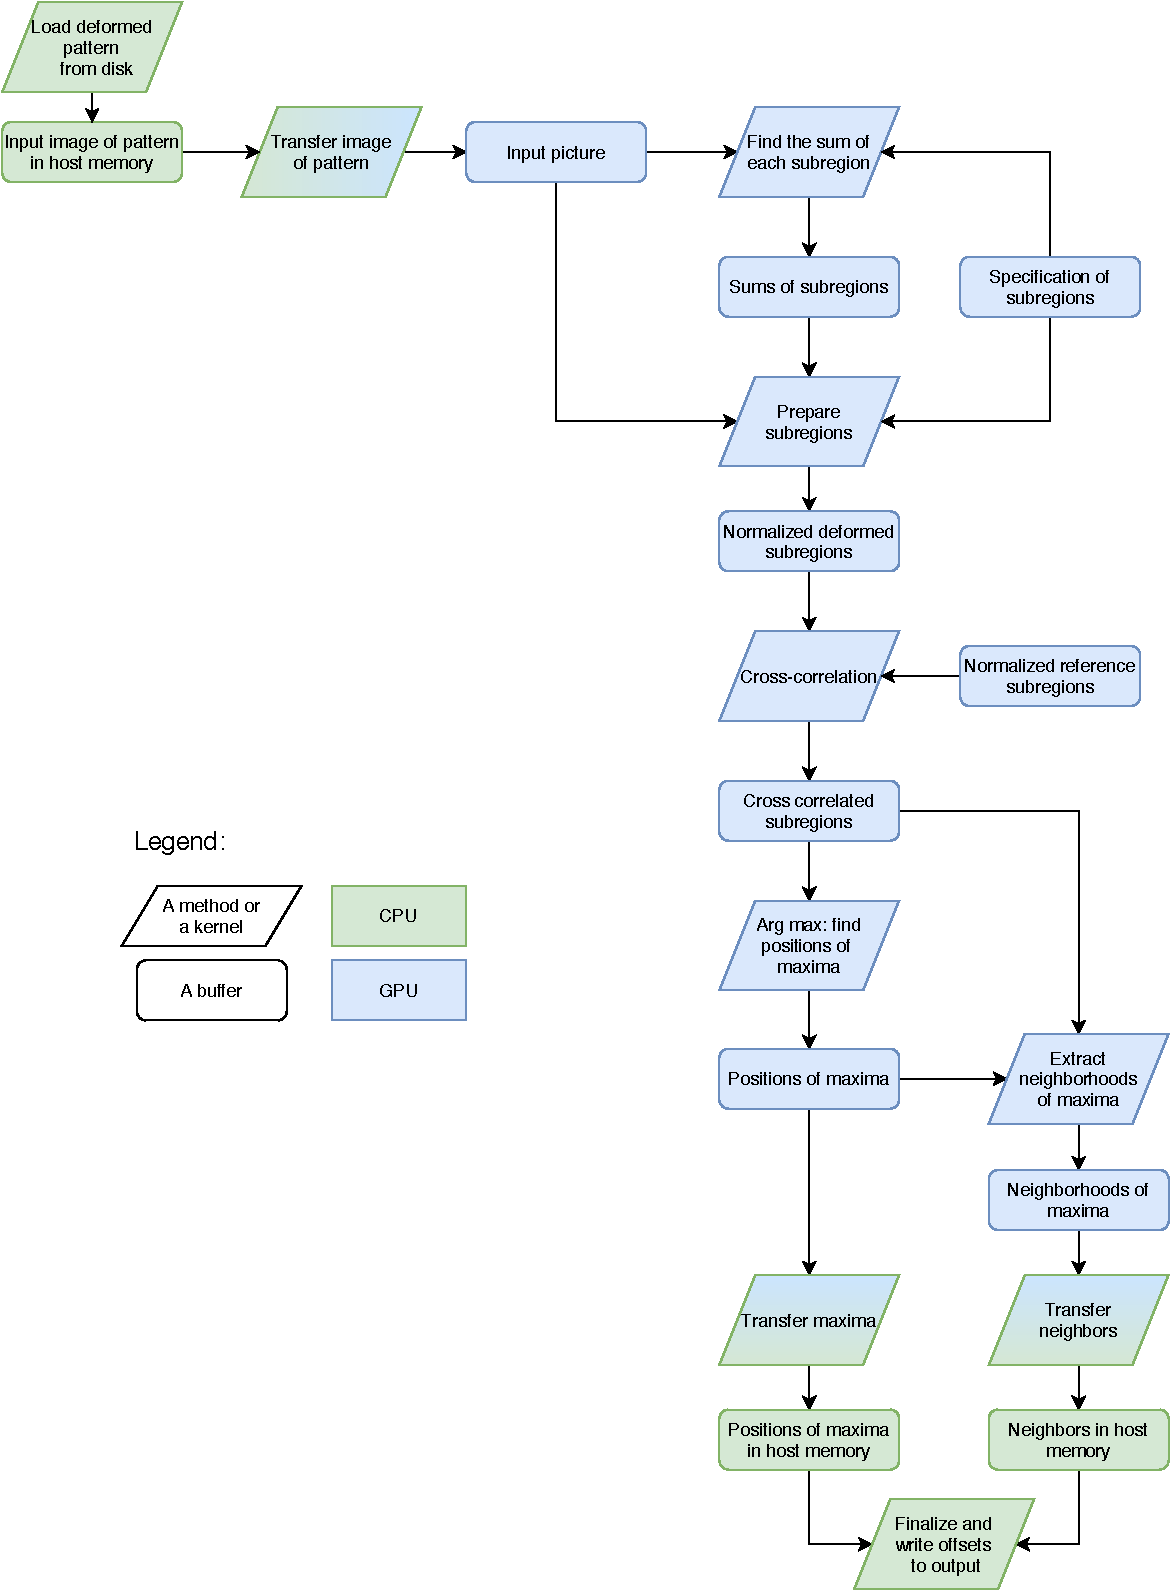
\includegraphics[width=\textwidth]{img/overview}
	\caption{Processing of one deformed pattern.}
	\label{overview}
\end{figure}

\Cref{overview} shows the data flow of the implementation and its decomposition into kernels. The processing starts with loading an image of a pattern from disk and its transfer to GPU. We transfer the whole pattern, as opposed to transferring only the subregions of interest.  Although we may end up copying data that the GPU never uses, this approach turned out to be better, because then we can utilize GPU when slicing the pattern into subregions. Moreover, we expect the regions to overlap in typical use case, so transferring the whole pattern copies less data.

The image is represented as an array of all the pixels in row--major order. Each pixel is an unsigned integer. 

Next, we need to prepare the data for cross--correlation --- slice the image of deformed pattern to subregions and normalize them by subtracting the respective means. It is done in two kernels: the first one computes the sum of pixels of each subregion using parallel reduction. The second kernel extracts the subregions from the pattern, so that they are organized one after another in the output buffer: first, there all the pixels of the first subregion in row--major order, then all the pixels from the second and so on. Moreover, the kernel uses the sums from the first kernel to compute the mean for each region and subtracts it from each pixel of respective subregion.

The following part cross--correlates the normalized deformed subregions with reference ones. Since each deformed pattern is compared to the same reference, we pre-compute it and store it in a buffer on the GPU before loading the first deformed pattern.

Then, we analyze the result of the cross--correlation --- we find where is the maximum of each subregion using parallel reduction. The result is an array of coordinates of the maximum values (we are not interested in the values themselves). The next kernel then extracts a square shaped neighborhood of each maximum into one continuous buffer, so it can be transferred to the CPU memory together with the positions of the maxima.

The last part of the algorithm fits a continuous quadratic function to the neighborhood and then finds its maximum. We did not implement it for GPU, because it is not computationally demanding. It processes only a small neighborhood compared to the expected size of subregions. That also makes it cheap to transfer the maxima and neighborhoods from GPU to finish the computation on CPU and write the results to the output.

The decomposition into kernels is mostly determined by the need of global barriers. Both finding of sum and argmax use parallel reduction, which has to fully finish before any of its results are complete. The kernel that extracts the subregions from the pattern is necessary, to simplify the cross--correlation and allow usage of third party libraries (see \cref{fft}, where the implementation of cross--correlation is explained).

\Cref{overview} also shows which parts are done on CPU and which on GPU. It is desirable that we parallelize those tasks, so that GPU is fully utilized and does not wait on CPU work.

 Parallelization of CPU and GPU parts



\section{Sum computation}
\section{Cross--correlation}
\subsection{Fourier transform}
\label{fft}
\section{Least squares implementation}